\documentclass[
  man,
  floatsintext,
  longtable,
  nolmodern,
  notxfonts,
  notimes,
  colorlinks=true,linkcolor=blue,citecolor=blue,urlcolor=blue]{apa7}

\usepackage{amsmath}
\usepackage{amssymb}



\usepackage[bidi=default]{babel}
\babelprovide[main,import]{english}


% get rid of language-specific shorthands (see #6817):
\let\LanguageShortHands\languageshorthands
\def\languageshorthands#1{}

\RequirePackage{longtable}
\RequirePackage{threeparttablex}

\makeatletter
\renewcommand{\paragraph}{\@startsection{paragraph}{4}{\parindent}%
	{0\baselineskip \@plus 0.2ex \@minus 0.2ex}%
	{-.5em}%
	{\normalfont\normalsize\bfseries\typesectitle}}

\renewcommand{\subparagraph}[1]{\@startsection{subparagraph}{5}{0.5em}%
	{0\baselineskip \@plus 0.2ex \@minus 0.2ex}%
	{-\z@\relax}%
	{\normalfont\normalsize\bfseries\itshape\hspace{\parindent}{#1}\textit{\addperi}}{\relax}}
\makeatother




\usepackage{longtable, booktabs, multirow, multicol, colortbl, hhline, caption, array, float, xpatch}
\usepackage{subcaption}


\renewcommand\thesubfigure{\Alph{subfigure}}
\setcounter{topnumber}{2}
\setcounter{bottomnumber}{2}
\setcounter{totalnumber}{4}
\renewcommand{\topfraction}{0.85}
\renewcommand{\bottomfraction}{0.85}
\renewcommand{\textfraction}{0.15}
\renewcommand{\floatpagefraction}{0.7}

\usepackage{tcolorbox}
\tcbuselibrary{listings,theorems, breakable, skins}
\usepackage{fontawesome5}

\definecolor{quarto-callout-color}{HTML}{909090}
\definecolor{quarto-callout-note-color}{HTML}{0758E5}
\definecolor{quarto-callout-important-color}{HTML}{CC1914}
\definecolor{quarto-callout-warning-color}{HTML}{EB9113}
\definecolor{quarto-callout-tip-color}{HTML}{00A047}
\definecolor{quarto-callout-caution-color}{HTML}{FC5300}
\definecolor{quarto-callout-color-frame}{HTML}{ACACAC}
\definecolor{quarto-callout-note-color-frame}{HTML}{4582EC}
\definecolor{quarto-callout-important-color-frame}{HTML}{D9534F}
\definecolor{quarto-callout-warning-color-frame}{HTML}{F0AD4E}
\definecolor{quarto-callout-tip-color-frame}{HTML}{02B875}
\definecolor{quarto-callout-caution-color-frame}{HTML}{FD7E14}

%\newlength\Oldarrayrulewidth
%\newlength\Oldtabcolsep


\usepackage{hyperref}




\providecommand{\tightlist}{%
  \setlength{\itemsep}{0pt}\setlength{\parskip}{0pt}}
\usepackage{longtable,booktabs,array}
\usepackage{calc} % for calculating minipage widths
% Correct order of tables after \paragraph or \subparagraph
\usepackage{etoolbox}
\makeatletter
\patchcmd\longtable{\par}{\if@noskipsec\mbox{}\fi\par}{}{}
\makeatother
% Allow footnotes in longtable head/foot
\IfFileExists{footnotehyper.sty}{\usepackage{footnotehyper}}{\usepackage{footnote}}
\makesavenoteenv{longtable}

\usepackage{graphicx}
\makeatletter
\newsavebox\pandoc@box
\newcommand*\pandocbounded[1]{% scales image to fit in text height/width
  \sbox\pandoc@box{#1}%
  \Gscale@div\@tempa{\textheight}{\dimexpr\ht\pandoc@box+\dp\pandoc@box\relax}%
  \Gscale@div\@tempb{\linewidth}{\wd\pandoc@box}%
  \ifdim\@tempb\p@<\@tempa\p@\let\@tempa\@tempb\fi% select the smaller of both
  \ifdim\@tempa\p@<\p@\scalebox{\@tempa}{\usebox\pandoc@box}%
  \else\usebox{\pandoc@box}%
  \fi%
}
% Set default figure placement to htbp
\def\fps@figure{htbp}
\makeatother


% definitions for citeproc citations
\NewDocumentCommand\citeproctext{}{}
\NewDocumentCommand\citeproc{mm}{%
  \begingroup\def\citeproctext{#2}\cite{#1}\endgroup}
\makeatletter
 % allow citations to break across lines
 \let\@cite@ofmt\@firstofone
 % avoid brackets around text for \cite:
 \def\@biblabel#1{}
 \def\@cite#1#2{{#1\if@tempswa , #2\fi}}
\makeatother
\newlength{\cslhangindent}
\setlength{\cslhangindent}{1.5em}
\newlength{\csllabelwidth}
\setlength{\csllabelwidth}{3em}
\newenvironment{CSLReferences}[2] % #1 hanging-indent, #2 entry-spacing
 {\begin{list}{}{%
  \setlength{\itemindent}{0pt}
  \setlength{\leftmargin}{0pt}
  \setlength{\parsep}{0pt}
  % turn on hanging indent if param 1 is 1
  \ifodd #1
   \setlength{\leftmargin}{\cslhangindent}
   \setlength{\itemindent}{-1\cslhangindent}
  \fi
  % set entry spacing
  \setlength{\itemsep}{#2\baselineskip}}}
 {\end{list}}
\usepackage{calc}
\newcommand{\CSLBlock}[1]{\hfill\break\parbox[t]{\linewidth}{\strut\ignorespaces#1\strut}}
\newcommand{\CSLLeftMargin}[1]{\parbox[t]{\csllabelwidth}{\strut#1\strut}}
\newcommand{\CSLRightInline}[1]{\parbox[t]{\linewidth - \csllabelwidth}{\strut#1\strut}}
\newcommand{\CSLIndent}[1]{\hspace{\cslhangindent}#1}





\usepackage{newtx}

\defaultfontfeatures{Scale=MatchLowercase}
\defaultfontfeatures[\rmfamily]{Ligatures=TeX,Scale=1}





\title{Replication Project for the paper Immigration and Crime: An
International Perspective}


\shorttitle{Replication Project for the paper Immigration and Crime: An
International Perspective}


\usepackage{etoolbox}








\authorsnames{Yu-Chiao Tseng 400778357,Tawanda Nhundu 400744073}





\affiliation{
{Hochschule Fresenius}}




\leftheader{400778357 and 400744073}



\abstract{This is a report of a replication study focusing on the paper
titled Immigration and Crime: An International Perspective. It aims to
authenticate the results of 2 figures of the authors by attempting to
replicate using the programming language R.The replication process has
been assisted by AI in code design with the final results to be
published on GitHub.This report will cover all the steps to complete the
report, the codes used and the problems encountered during the
replication. }



\authornote{ 

\par{       }
\par{Correspondence concerning this article should be addressed
to Yu-Chiao Tseng
400778357, Email: \href{mailto:tseng.yu-chiao@stud.hs-fresenius.de}{tseng.yu-chiao@stud.hs-fresenius.de}Tawanda
Nhundu
400744073, Email: \href{mailto:nhundu.tawanda@stud.hs-fresenius.de}{nhundu.tawanda@stud.hs-fresenius.de}}
}

\makeatletter
\let\endoldlt\endlongtable
\def\endlongtable{
\hline
\endoldlt
}
\makeatother

\urlstyle{same}



\pagestyle{empty}
\makeatletter
\@ifpackageloaded{caption}{}{\usepackage{caption}}
\AtBeginDocument{%
\ifdefined\contentsname
  \renewcommand*\contentsname{Table of contents}
\else
  \newcommand\contentsname{Table of contents}
\fi
\ifdefined\listfigurename
  \renewcommand*\listfigurename{List of Figures}
\else
  \newcommand\listfigurename{List of Figures}
\fi
\ifdefined\listtablename
  \renewcommand*\listtablename{List of Tables}
\else
  \newcommand\listtablename{List of Tables}
\fi
\ifdefined\figurename
  \renewcommand*\figurename{Figure}
\else
  \newcommand\figurename{Figure}
\fi
\ifdefined\tablename
  \renewcommand*\tablename{Table}
\else
  \newcommand\tablename{Table}
\fi
}
\@ifpackageloaded{float}{}{\usepackage{float}}
\floatstyle{ruled}
\@ifundefined{c@chapter}{\newfloat{codelisting}{h}{lop}}{\newfloat{codelisting}{h}{lop}[chapter]}
\floatname{codelisting}{Listing}
\newcommand*\listoflistings{\listof{codelisting}{List of Listings}}
\makeatother
\makeatletter
\makeatother
\makeatletter
\@ifpackageloaded{caption}{}{\usepackage{caption}}
\@ifpackageloaded{subcaption}{}{\usepackage{subcaption}}
\makeatother

% From https://tex.stackexchange.com/a/645996/211326
%%% apa7 doesn't want to add appendix section titles in the toc
%%% let's make it do it
\makeatletter
\xpatchcmd{\appendix}
  {\par}
  {\addcontentsline{toc}{section}{\@currentlabelname}\par}
  {}{}
\makeatother

%% Disable longtable counter
%% https://tex.stackexchange.com/a/248395/211326

\usepackage{etoolbox}

\makeatletter
\patchcmd{\LT@caption}
  {\bgroup}
  {\bgroup\global\LTpatch@captiontrue}
  {}{}
\patchcmd{\longtable}
  {\par}
  {\par\global\LTpatch@captionfalse}
  {}{}
\apptocmd{\endlongtable}
  {\ifLTpatch@caption\else\addtocounter{table}{-1}\fi}
  {}{}
\newif\ifLTpatch@caption
\makeatother

\begin{document}

\maketitle




\setlength\LTleft{0pt}




\section{Introduction}\label{introduction}

The goal of this project is to conduct a replication study. Our group
selected the paper from Olivier Marie and Paolo Pinotti (2024) which
explored the association between immigration and crime in the Journal of
Economic Perspectives. They found that an increase in the share of
immigrants was not accompanied by an increase in the global murder rate.

We will discuss more detail the process of finding papers, how we used R
to complete this replication study, the challenges we encountered, and
how we published our report on GitHub. Lastly, we will summarize the
learning process.

\section{Motivation for Replication}\label{motivation-for-replication}

Academic research nowadays values transparency and credibility, and
replication studies are an important way to verify these.There are some
researchers manipulate data to achieve the results they want, and
replication studies can confirm that the author's research results are
not accidental or the result of incorrect analysis method. The
importance of research in science and academic knowledge is
self-evident. According to Bouter \& ter\,Riet (2021) replication is
divided into three different levels. First, reanalysis of the original
study by re‑running their exact code and dataset, to verify that the
published figures and tables can be fully reproduced. The second one is
direct replication which means replicate with new data but the same
research protocol. The third one is conceptual replication, researchers
use new data with the modified research protocol and same research
question. In the project I think we did re‑analysis, we used the data
provided by the authors and the same data analysis plan.Using the world
bank data as weight can be a conceptual replication. Bouter \& ter\,Riet
mentioned that by varying data sources or methods, conceptual
replications can reveal whether a finding can be use in different
context and proof it validity and generalizability. In contrast,
reanalyses or direct replications which rely on the same dataset or same
procedures might reproduce the flaws that were present in the original
study.

(\citeproc{ref-bouter2021a}{Bouter \& Riet, 2021})

\section{Finding a paper}\label{finding-a-paper}

We selected two papers, ``Inside the Box'' and ``Immigration and Crime''
at the beginning. The first one was written by an author who used R to
do most of his work, so the professor suggested that we choose another
one. In the article ``Immigration and Crime'', the author used Stata for
coding. The article explored the relationship between immigration and
crime. Living abroad as students, we felt that the increase in
immigration in many countries in recent years has brought benefits such
as filling the labor gap in developed countries, but it has also caused
many conflicts between immigrants and locals. Many people believe that
immigrants cause public security problems and have low tolerance for
them. Seeing this trend, enhanced our interest in this topic, and we
hope to learn more about the content of the article and how the author
conducts statistical analysis and explores this issue.

The authors Olivier Marie and Paolo Pinotti cleaned, merged, and
statistically analyzed the United Nations' immigration and crime data to
explore whether there is a significant correlation between immigration
and crime. They also referred to other studies to further explore
whether obtaining legal status reduces the tendency to commit crimes. We
chose Figure 2 and Figure 4 for replication. First, we read the author's
README file and Stata code to confirm the feasibility and verify whether
the data set can be accessed from the websites they provided.

\section{Figure 2 Top Replication
Process}\label{figure-2-top-replication-process}

Figure 2 is composed of two figures, the first one is a double y-axis
graph, showing the long-term trend of the ``proportion of immigrants to
the total population'' gray line and the ``murder rate'' blue line in 55
countries (1990-2019). The second figure is a scatter plot, showing how
much the ``number of immigrants'' in each country changed from 1990 to
2019 and how much the ``murder rate'' changed during the same period
(calculated in logarithms).

\phantomsection\label{fig:original}
\textbf{Figure~1.}\\
\emph{Original graph of Figure~2}

\begin{center}
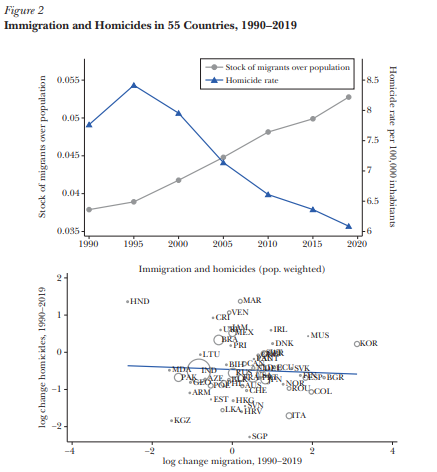
\includegraphics[width=0.8\linewidth,height=\textheight,keepaspectratio]{fig/Original.png}
\end{center}

(\citeproc{ref-marie2024}{Marie \& Pinotti, 2024})

\textbf{Figure~2.}\\
\emph{Original Stata code for Figure 2 top}

\begin{center}
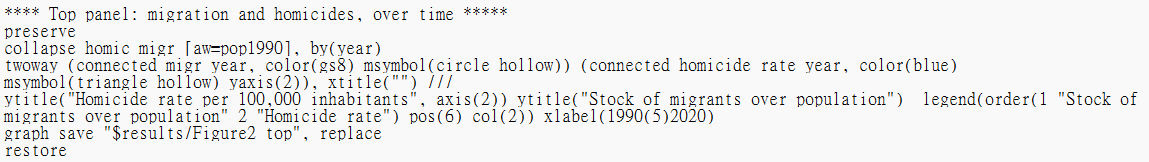
\includegraphics[width=0.8\linewidth,height=\textheight,keepaspectratio]{fig/statatop.png}
\end{center}

This part relies on chatgpt's explanation to understand the meaning of
each code collapse homic migr {[}aw=pop1990{]}, by(year) is grouped by
year, and the variables homic and migr are weighted averaged (weight is
pop1990), Two-way connected plot is a two-line graph, connected migr
year, color(gs8) msymbol(circle\_hollow) draws the first line (left Y
axis), connected homicide\_rate year, color(blue)
msymbol(triangle\_hollow) yaxis(2) draws the second line (right Y axis).
Then I created a new file in R and saved the data provided by the
author.

ChatGPT guided me step by step to reproduce this grpah in R.

\pandocbounded{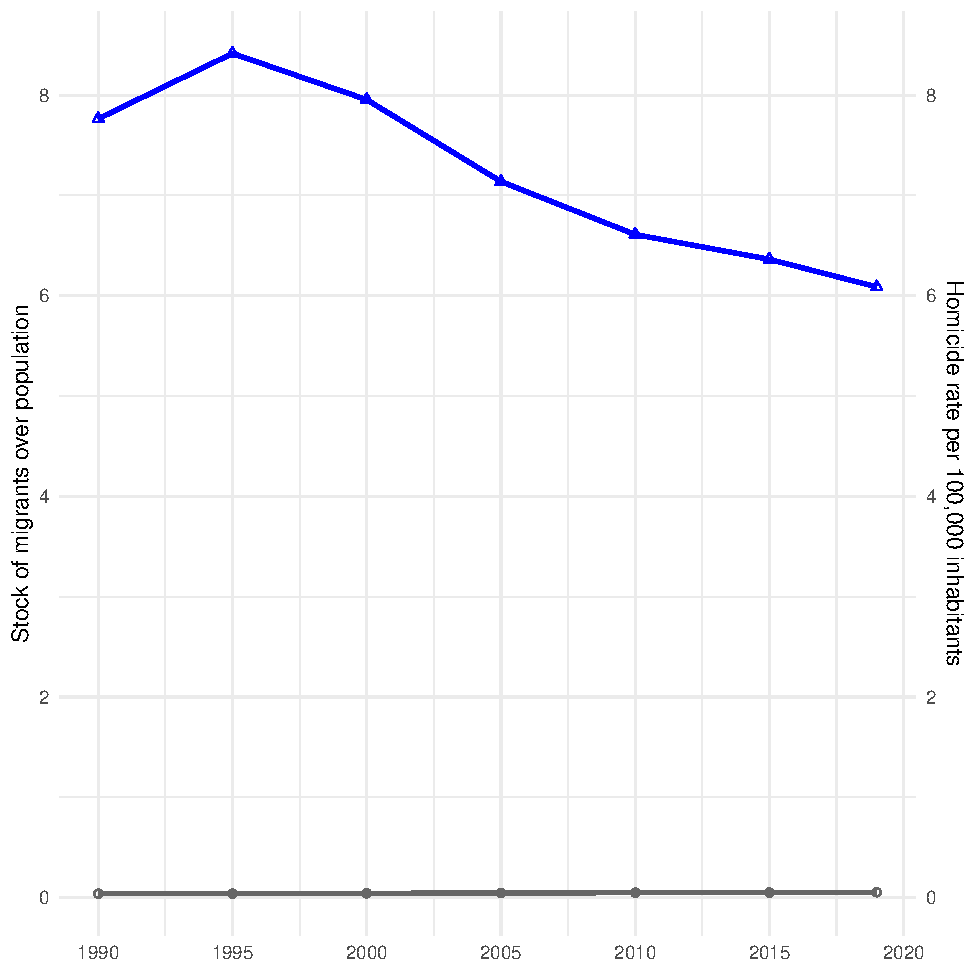
\includegraphics[keepaspectratio]{Replication-Report_files/figure-pdf/unnamed-chunk-1-1.pdf}}

(OpenAI, 2025)

Here is the first problem

As we can see, the gray line on the graph made according to the above
code is almost attached to the bottom of the graph. I asked Chatgpt, and
it said that the gray ``immigrant proportion'' line is always close to
0. This is because the dual Y axes of ggplot2 are not truly
``independently scaled'', but share a set of numerical spaces. hom\_w
(murder rate) is about 6 to 9, and migr\_w (immigrant proportion) is
about 0.03 to 0.055. After looking at the graph, I also noticed that the
scales on both sides of my graph are 0-8, while the scale on the left
side of the author's graph is 0.035-0.055.

Then ChatGPT Offered Solution:

\phantomsection\label{fig:S2}
\textbf{Figure~3.}\\
\emph{Soluction for flat gray line}

\begin{center}
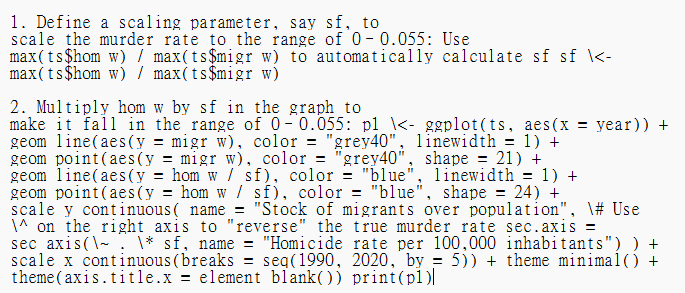
\includegraphics[width=0.8\linewidth,height=\textheight,keepaspectratio]{fig/S2.png}
\end{center}

Here I follow the instruction, use y = hom\_w / sf when drawing the blue
line (equivalent to ``compressing'' the murder rate to the small
interval of the proportion of immigrants), Then use
sec\_axis(\textasciitilde{} . * sf) to ``expand'' the label on the right
back to the true murder rate value. After following the steps of
chatgpt, the two lines are in the correct position. Lastly, I corrected
the scales on both sides to 0.035-0.055 on the left axis and 6-8.5 on
the right axis.

\pandocbounded{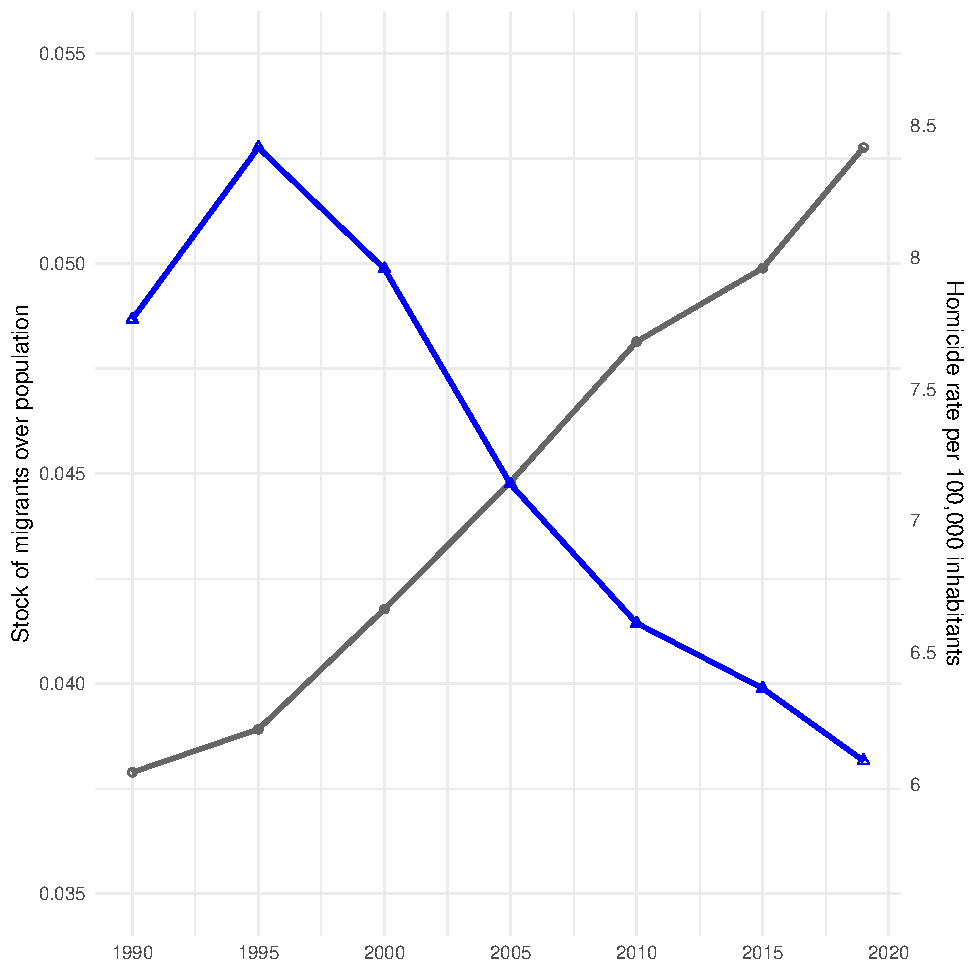
\includegraphics[keepaspectratio]{Replication-Report_files/figure-pdf/unnamed-chunk-2-1.pdf}}

After following the steps of ChatGPT, the two lines are now in the
correct position. Lastly, I corrected the scales on both sides to
0.035-0.055 on the left axis and 6-8.5 on the right axis to make it more
alike to original one.

I also noticed that the gray line ended up closer to 8.5, while the
original graph looked between 8 and 8.5. I asked ChatGPT and checked
three things according to it's instructions. 1. Did I draw 2020 ? 2.
Confirm that migr\_pop is a proportion, not a number of people 3.
Re-ensure that the weighted average uses the pop1990 column I checked
all of them, but the graph did not change. ChatGPT said that it might be
that the weighting method in Stata is slightly different from the
implementation details in R, or that the original graph was slightly
adjusted manually when it was published.(OpenAI, 2025) I remember
learning in the course last semester that the key to doing replication
is to be able to reproduce the results and trends that the chart wants
to present after following the code provided by the author and the same
method. In this graph, the direction of the lines is consistent with the
changes (immigration increased, murders decreased), and the values are
roughly in the same area, with no obvious misalignment or data errors. I
think the points where the two lines fall and where they intersect are
not significantly different from the original graph, so I believe this
is a successful replication.

\subsection{Discussion on Figure 2
top}\label{discussion-on-figure-2-top}

Figure 2 top graph uses United Nations immigration data. I think the
author could be more precise on that. Did they use International migrant
stock from United Nations data or Total population, or both? At first, I
compared the numbers on the data and the website, and found that there
was a slight difference between the total population on the website and
the file provided by the author. For example, the total population of
Australia in 1990 was 16960.600 in the author's data and 17126.298 on
the website. The total population of Armenia in 1990 was 3538.164, and
3552.128 on the website. I thought that this might be because the data
on the website had been updated. If the difference was not big, I
thought the data provided by the author was credible, so I directly used
the author's data for replication. Later, I further wanted to confirm
where the number of migr\_pop in the author's file came from, but I
couldn't calculate a similar number. Finally, I realized the problem is
that I downloaded the latest version of the data, and the author used
the 2020 version. The latest version is Armenia 1990 Total population at
mid-year 3552.128, migrant stock 433541. The version used by the author,
Armenia 1990 Total population at mid-year 3538.164, migrant stock has
been updated a lot, which led to my calculation of 433541/3552.128
≈0.1225, not ≈0.186. Another issue was the numbers for migrant stock are
missing from the file provided by the authors; it has only the author's
own calculation of migr\_pop 0.186195165. I think the author's readme
file can include the file year used and how migr\_pop is calculated.
This can improve the overall transparency and credibility of the
research and reduce disputes over errors caused by different versions.

\section{Figure 2 Bottom Replication
Process}\label{figure-2-bottom-replication-process}

The bottom plot is the logarithmic change scatter plot + weighted
regression line for 1990 vs.~2019. X axis: log change migration, Y axis:
log change homicides.

\phantomsection\label{fig:statabottom}
\textbf{Figure~4.}\\
\emph{the original Stata code for Figure 2 bottom}

\begin{center}
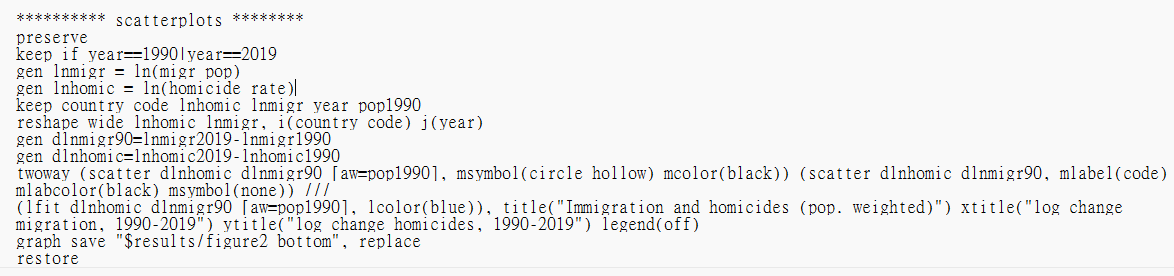
\includegraphics[width=0.8\linewidth,height=\textheight,keepaspectratio]{fig/statabottom.png}
\end{center}

Same I followed the instructions of ChatGPT to do the steps, first
select 1990 and 2019 from the original data

\begin{verbatim}
# A tibble: 6 x 6
  code  pop1990 ln_migr_1990 ln_migr_2019 ln_homic_1990 ln_homic_2019
  <chr>   <dbl>        <dbl>        <dbl>         <dbl>         <dbl>
1 ARM     3538.        -1.68        -2.74         1.62         0.525 
2 AUS    16961.        -1.46        -1.21         0.793       -0.117 
3 AUT     7724.        -2.28        -1.62         0.140       -0.0305
4 AZE     7243.        -3.00        -3.68         1.51         0.788 
5 BLR    10151.        -2.10        -2.18         1.61         0.871 
6 BIH     4463.        -4.38        -4.53         0.495        0.157 
\end{verbatim}

\begin{verbatim}
tibble [55 x 6] (S3: tbl_df/tbl/data.frame)
 $ code         : chr [1:55] "ARM" "AUS" "AUT" "AZE" ...
  ..- attr(*, "label")= chr "code"
  ..- attr(*, "format.stata")= chr "%9s"
 $ pop1990      : num [1:55] 3538 16961 7724 7243 10151 ...
  ..- attr(*, "format.stata")= chr "%9.0g"
 $ ln_migr_1990 : num [1:55] -1.68 -1.46 -2.28 -3 -2.1 ...
  ..- attr(*, "format.stata")= chr "%9.0g"
 $ ln_migr_2019 : num [1:55] -2.74 -1.21 -1.62 -3.68 -2.18 ...
  ..- attr(*, "format.stata")= chr "%9.0g"
 $ ln_homic_1990: num [1:55] 1.615 0.793 0.14 1.513 1.609 ...
  ..- attr(*, "label")= chr "homicide_rate"
  ..- attr(*, "format.stata")= chr "%10.0g"
 $ ln_homic_2019: num [1:55] 0.5247 -0.1165 -0.0305 0.7885 0.8713 ...
  ..- attr(*, "label")= chr "homicide_rate"
  ..- attr(*, "format.stata")= chr "%10.0g"
\end{verbatim}

\begin{verbatim}
Warning in geom_text_repel(aes(label = code), linewidth = 3): Ignoring unknown
parameters: `linewidth`
\end{verbatim}

\begin{verbatim}
`geom_smooth()` using formula = 'y ~ x'
\end{verbatim}

\pandocbounded{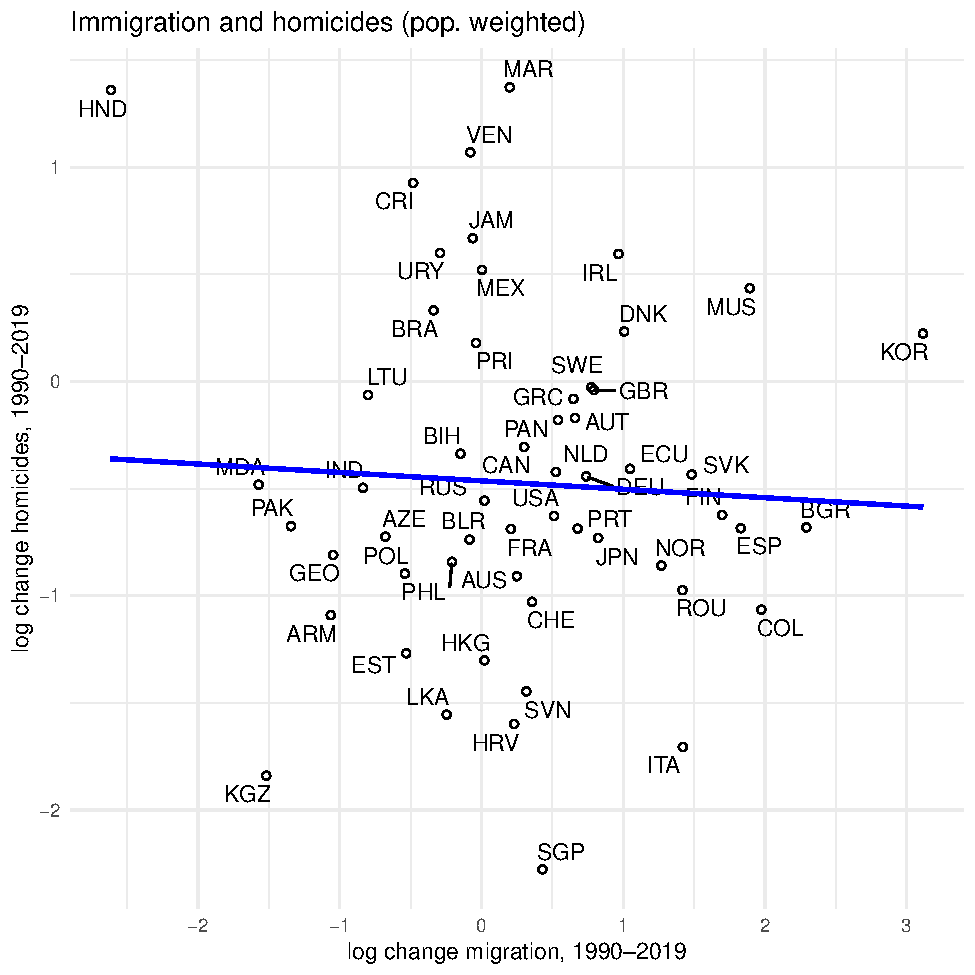
\includegraphics[keepaspectratio]{Replication-Report_files/figure-pdf/unnamed-chunk-3-1.pdf}}

It looks very similar to the original image, and then I adjusted the
scale.

\begin{verbatim}
`geom_smooth()` using formula = 'y ~ x'
\end{verbatim}

\begin{verbatim}
Warning: Removed 1 row containing non-finite outside the scale range
(`stat_smooth()`).
\end{verbatim}

\begin{verbatim}
Warning: Removed 1 row containing missing values or values outside the scale range
(`geom_point()`).
\end{verbatim}

\begin{verbatim}
Warning: Removed 1 row containing missing values or values outside the scale range
(`geom_text_repel()`).
\end{verbatim}

\pandocbounded{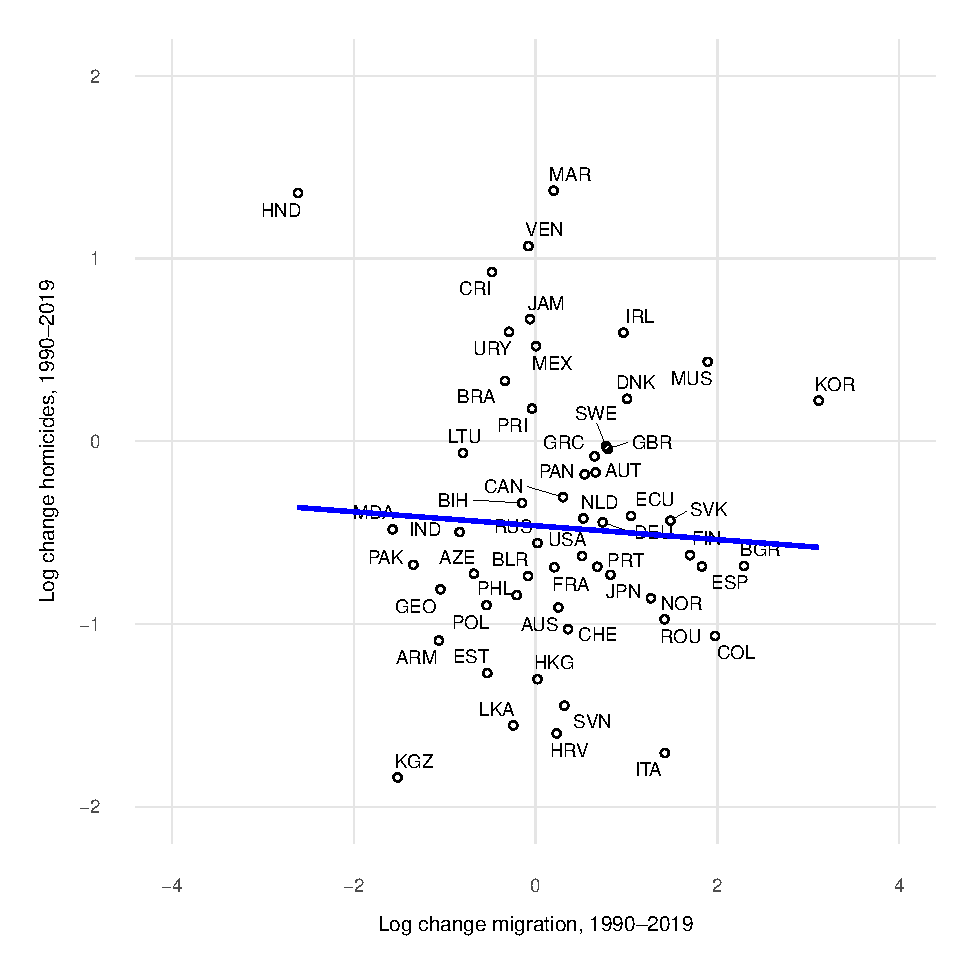
\includegraphics[keepaspectratio]{Replication-Report_files/figure-pdf/unnamed-chunk-4-1.pdf}}

Lastly, I use the code theme\_minimal(base\_size = 38) for the font size
adjustment. I think this graph shares the same idea that the author
wants to present in the paper. There is a nearly horizontal regression
line, and most countries are concentrated between -1 and 1 on the X
axis. This means that the proportion of immigrants and the murder rate
in most countries have not experienced a huge change. If more immigrants
lead to higher crime, there will be a cluster in the upper right corner
of the graph. However, the graph shows that there is no consistent trend
or causal relationship between changes in immigration and changes in
murder rates.

\section{Using World Bank population data as
weight}\label{using-world-bank-population-data-as-weight}

Because the group before us had some data generation problems, they
didn't seem to use the data used by the author, but the graph was
produced. The professor said that their data might be generated by
ChatGPT itself, and then said that they could go to the World Bank to
find the data they needed. At that time, I thought I had to use the
World Bank data, so I used the World Bank data to make the second graph.
But I didn't give ChatGPT instructions clear enough; I just said that I
wanted to use the World Bank population data to make a new graph.So
ChatGPT gave me the code:

\begin{verbatim}
Warning: There was 1 warning in `mutate()`.
i In argument: `code = countrycode(iso2c, "iso2c", "iso3c")`.
Caused by warning:
! Some values were not matched unambiguously: JG, XK
\end{verbatim}

\pandocbounded{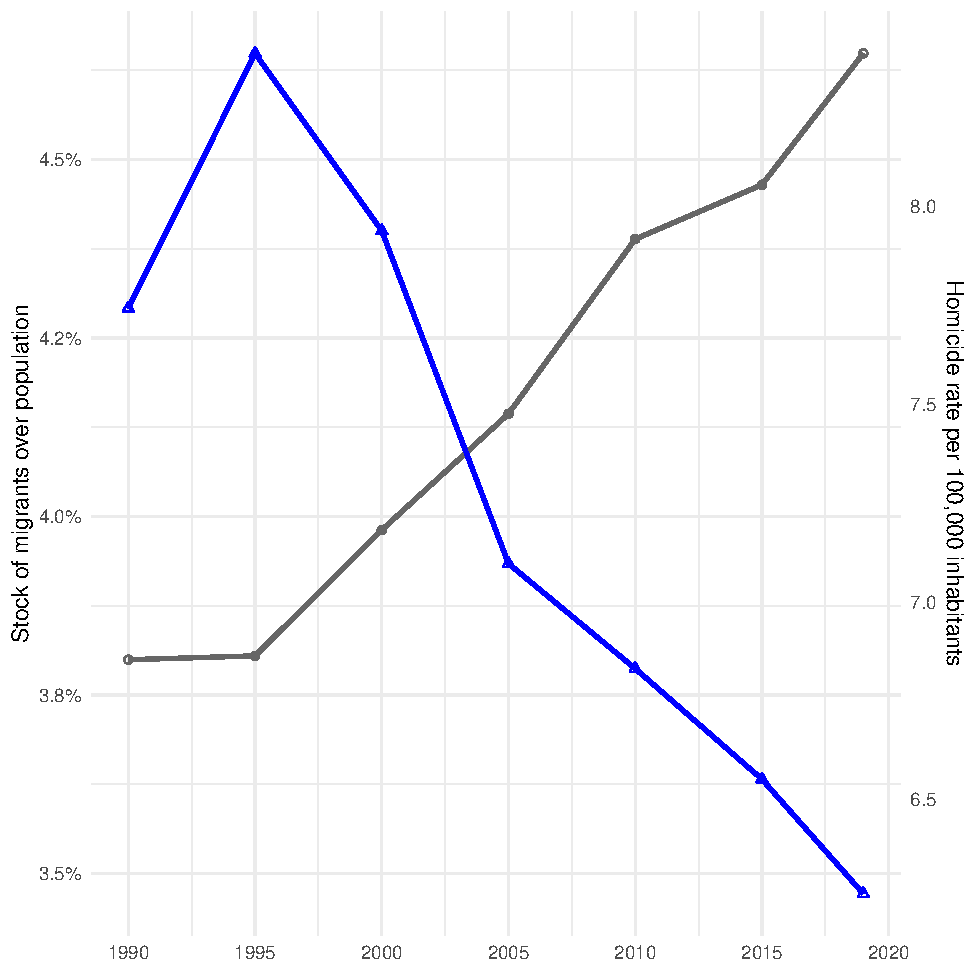
\includegraphics[keepaspectratio]{Replication-Report_files/figure-pdf/unnamed-chunk-5-1.pdf}}

The step after merging had mistake

\phantomsection\label{fig:M1}
\textbf{Figure~5}\\
\emph{Mistake using incorrect weights}

\begin{center}
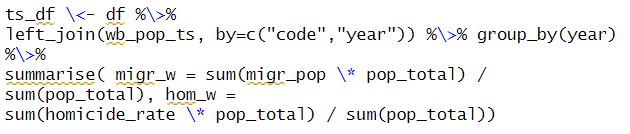
\includegraphics[width=1\linewidth,height=\textheight,keepaspectratio]{fig/M1.png}
\end{center}

Because I used the total population of all years from 1990 to 2019, what
I got was the ``weighted average of the population distribution of that
year'', which means that the weights change every year. Actually, I
don't need the total population of all years from 1990 to 2019. I only
need to replace the 1990 population (pop1990) with World Bank's data,
because the author used only the 1990 population (pop1990) as the weight
for all periods.

Second time, I only used the 1990 population as the weight for the whole
period, and I still use the migr\_pop calculated by the author as a
share.

\pandocbounded{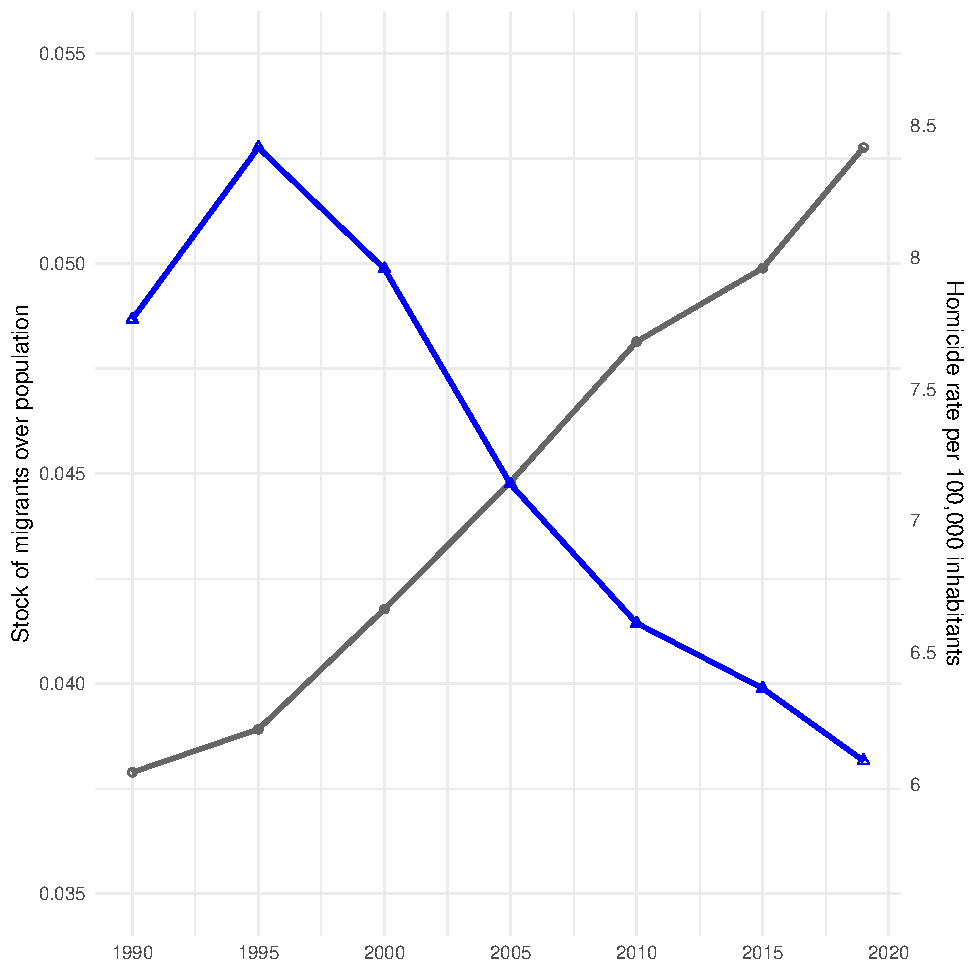
\includegraphics[keepaspectratio]{Replication-Report_files/figure-pdf/unnamed-chunk-6-1.pdf}}

\subsection{Discussion of using the data from the World Bank
incorrectly}\label{discussion-of-using-the-data-from-the-world-bank-incorrectly}

This graph looks very different from the last graph with mistakes, and
doesn't look significantly different from the first time I used the data
provided by the author.

This time, I used the data from the World Bank incorrectly and didn't
notice it at all. I intuitively thought that the graph looked different
only because I used the data from the World Bank. This caused me to be
embarrassed during my oral presentation.

\subsection{Problems with making a scatter plot at the
bottom}\label{problems-with-making-a-scatter-plot-at-the-bottom}

I also tried to make the bottom plot using the data from the World Bank,
but the problem I had was scatter plots did not appear.

\begin{verbatim}
Warning: There was 1 warning in `mutate()`.
i In argument: `code = countrycode(iso2c, "iso2c", "iso3c")`.
Caused by warning:
! Some values were not matched unambiguously: JG, XK
\end{verbatim}

\begin{verbatim}
`geom_smooth()` using formula = 'y ~ x'
\end{verbatim}

\begin{verbatim}
Warning: Removed 54 rows containing non-finite outside the scale range
(`stat_smooth()`).
\end{verbatim}

\begin{verbatim}
Warning: Removed 54 rows containing missing values or values outside the scale range
(`geom_point()`).
\end{verbatim}

\begin{verbatim}
Warning: Removed 54 rows containing missing values or values outside the scale range
(`geom_text_repel()`).
\end{verbatim}

\pandocbounded{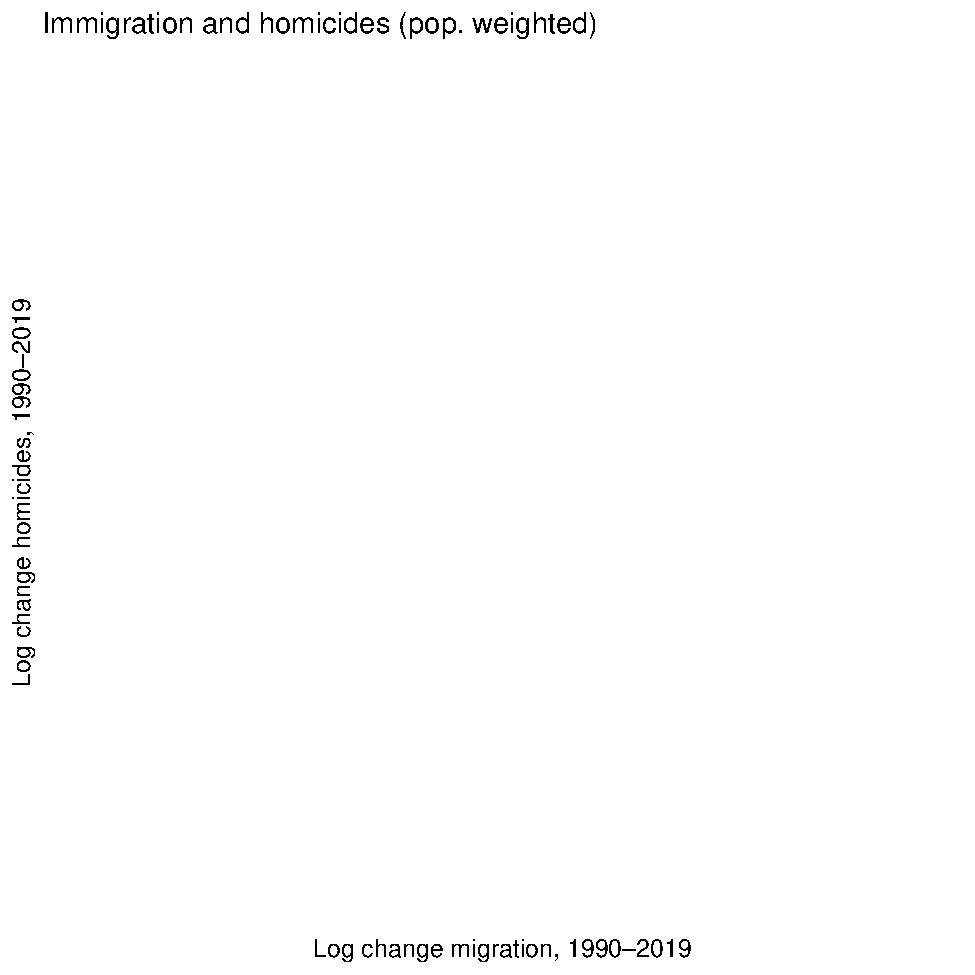
\includegraphics[keepaspectratio]{Replication-Report_files/figure-pdf/unnamed-chunk-7-1.pdf}}

I asked ChatGPT why this code can't make a scatter plot; the plot is
blank, there is no dots. At first, it couldn't find the reason, and
ChatGPT kept going around in circles. After hours, I changed the
conversation to a new chat room and re-posted the code. It finally works
and I just checked it step by step according to its instructions. For
example, check whether there are rows in the final data frame, and also
check setdiff(unique(df2\(code), unique(wb_pop\)code)) See which
countries are not in wb\_pop.

Finally, we found the problem, and ChatGPT explained it this way: The
problem is in the plot data frame, all rows corresponding to x =
dln\_migr or y = dln\_homic are treated as NA, so ggplot automatically
discards them.

The solution provided from ChatGPT is to keep only the columns I need
before pivoting

\phantomsection\label{fig:s1}
\textbf{Figure~6}\\
\emph{Solution for blank scattor plot}

\begin{center}
\includegraphics[width=0.8\linewidth,height=\textheight,keepaspectratio]{fig/s1.png}
\end{center}

(OpenAI, 2025)

After correcting according to the instructions, the scattered points
appeared.

\begin{verbatim}
   Min. 1st Qu.  Median    Mean 3rd Qu.    Max. 
-2.6146 -0.2811  0.2761  0.2960  0.8171  3.1155 
\end{verbatim}

\begin{verbatim}
    Min.  1st Qu.   Median     Mean  3rd Qu.     Max. 
-2.27727 -0.88754 -0.59014 -0.45285 -0.04651  1.37231 
\end{verbatim}

\begin{verbatim}
`geom_smooth()` using formula = 'y ~ x'
\end{verbatim}

\begin{verbatim}
Warning: Removed 1 row containing non-finite outside the scale range
(`stat_smooth()`).
\end{verbatim}

\begin{verbatim}
Warning: Removed 1 row containing missing values or values outside the scale range
(`geom_point()`).
\end{verbatim}

\begin{verbatim}
Warning: Removed 1 row containing missing values or values outside the scale range
(`geom_text_repel()`).
\end{verbatim}

\pandocbounded{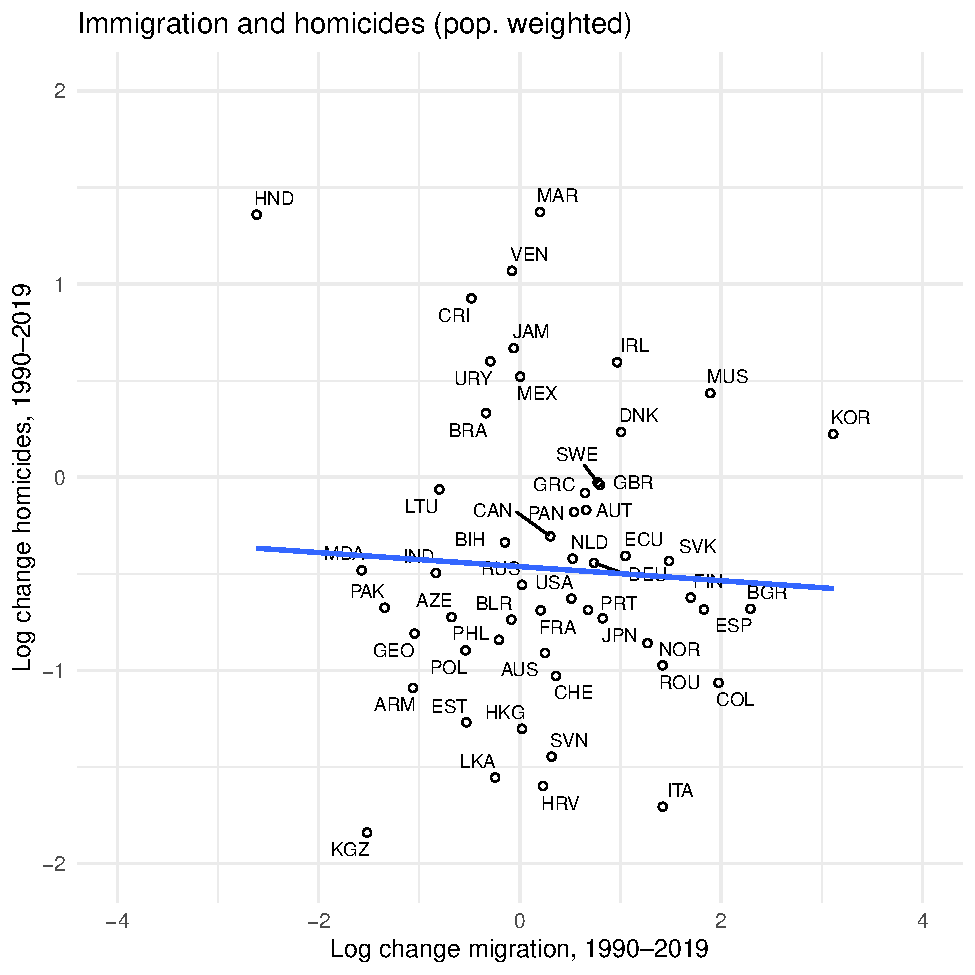
\includegraphics[keepaspectratio]{Replication-Report_files/figure-pdf/unnamed-chunk-8-1.pdf}}

\section{Figure 4}\label{figure-4}

Replication Figure 4, titled Summary of Estimates of the Impact of
Immigration on Crime attempts to look at the immigration on crime of 4
different countries. It attempts to do this by using a shift share
approach to determine whether increases in immigrants correlates with
increases in crime. This, however, does only provide casual estimates in
these two points. The paper uses two statistical methods in this figure,
ordinary least square estimates (OLS) and casual shift share estimates,
both with a 95 percent confidence intervals.

To look at the impact of immigration on crime, the paper does not
actually produce its own first-hand data, but rather analyses the data
from four other papers which looked at four countries respectively. The
countries and respective papers are Italy
(\citeproc{ref-bianchi2012}{Bianchi et al., 2012}), United Kingdom
(\citeproc{ref-bell2013}{Bell et al., 2013}), United States
(\citeproc{ref-spenkuch2010}{Spenkuch, 2010}) and Chile
(\citeproc{ref-ajzenman2020}{Ajzenman et al., 2020}). However, all four
papers gather their data with different methods, and therefore, the
analysis, and decision of how they the papers analysis these data in
down to the authors discretion, which became a problem for the data
replication which will be spoken about later.

\subsection{Original Figure 4}\label{original-figure-4}

The original figure 4 is a type of forest plot. It compares both the
relationship between immigration and crime looking at both effects on
property such as burglary or home owners increasing security and general
crime. As said before, because each of the for papers can use different
categorisations for what falls under these terms, this are statistical
estimations, with the choices of what falls under these categories left
to the authors discretion. Forest plots are powerful graphical displays
for meta-analyses and systematic reviews as they help summarise and
compare the results of multiple scientific studies. The plot helps to
visualise the estimated differences between many studies which is most
likely why the authors decided to use it here. Furthermore, within each
study, the authors were able to compare both the OLS and casual shift
shares. However, because these are estimates, this makes it a good
candidate to perform a replication study to avoid any biases from the
authors affecting their interpretation of their chosen studies results.

\phantomsection\label{fig:1}
\textbf{Figure~7}\\
\emph{Original graph of Figure~4}

\begin{center}
\pandocbounded{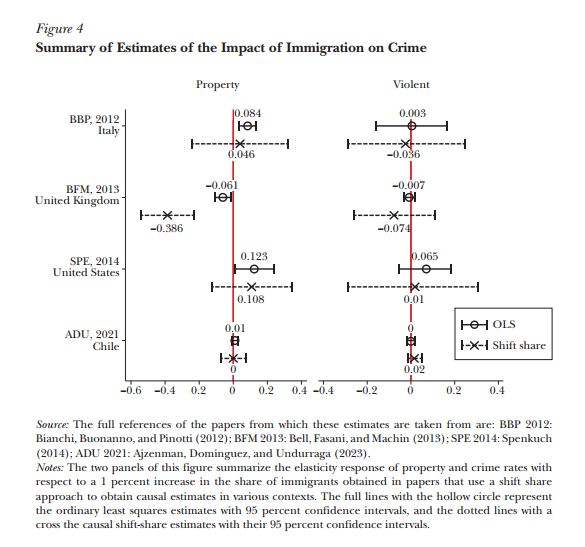
\includegraphics[keepaspectratio]{fig/1.jpeg}}
\end{center}

\subsection{Replication of Figure 4 from the Replication
Package}\label{replication-of-figure-4-from-the-replication-package}

Initially to confirm the feasibility of replicating the data, before
accessing the replication packages of the original four papers to do the
complete data replication, it was decided to first replicate the
author's data. Due to the fact that the authors performed their own
analysis, it was still necessary to confirm whether the authors
correctly produced their figures correctly from the data they provided
in their own replication package. Therefore, to confirm figure 4's
accuracy, first it was necessary to reproduce their figure. However, the
data used within their replication package was a Stata document rather
than a format that could be used directly in R. The Stata file relevant
to figure 4 was titled ``literature.dta''. The data was first uploaded
into the RStudio Cloud workspace for further analyses. Due to the file
being a Stata file, there was a two-fold reason for converting the data
into an Excel spreadsheet, one for personal sake, and the other due to
it not being a native Quatro file format. Therefore it was first
necessary to convert the data.

Fortunately, the steps to convert this file was not difficult with the
packages haven, writexl, dplyr and readxl this was achievable. This
brings the importance of knowing what the format of the data to be
analysed for a replication study is. There are many computer programming
languages, with various researchers deciding on what language to use
depending on what research they are doing. Fortunately at this time of
AI tools, it is much easier to figure out what the best means are to
change the data into a format usable y the programming tool you are
using. Gemini was also able to suggest the ways to use certain packages
to convert the data into a readable format. Initially the packages were
downloaded and used to read the data. Then, with writexl, the data was
successfully converted into an .xlsx file with the same ``literature''
name.

\begin{verbatim}
# A tibble: 6 x 6
  Paper_long                      Country Group         Coef   C_low C_high
  <chr>                           <chr>   <chr>        <dbl>   <dbl>  <dbl>
1 Bianchi Buonanno & Pinotti 2012 ITA     Immigration  0.046 -0.248   0.34 
2 Bianchi Buonanno & Pinotti 2012 ITA     Immigration  0.084  0.0291  0.139
3 Bianchi Buonanno & Pinotti 2012 ITA     Immigration  0.003 -0.162   0.168
4 Bianchi Buonanno & Pinotti 2012 ITA     Immigration -0.036 -0.313   0.241
5 Bell Fasani & Machin 2013       UK      Immigration -0.386 -0.545  -0.227
6 Bell Fasani & Machin 2013       UK      Immigration -0.061 -0.11   -0.012
\end{verbatim}

\phantomsection\label{fig:2}
\textbf{Figure~8.}\\
\emph{Table of the Stata File Titled literature}

\begin{center}
\pandocbounded{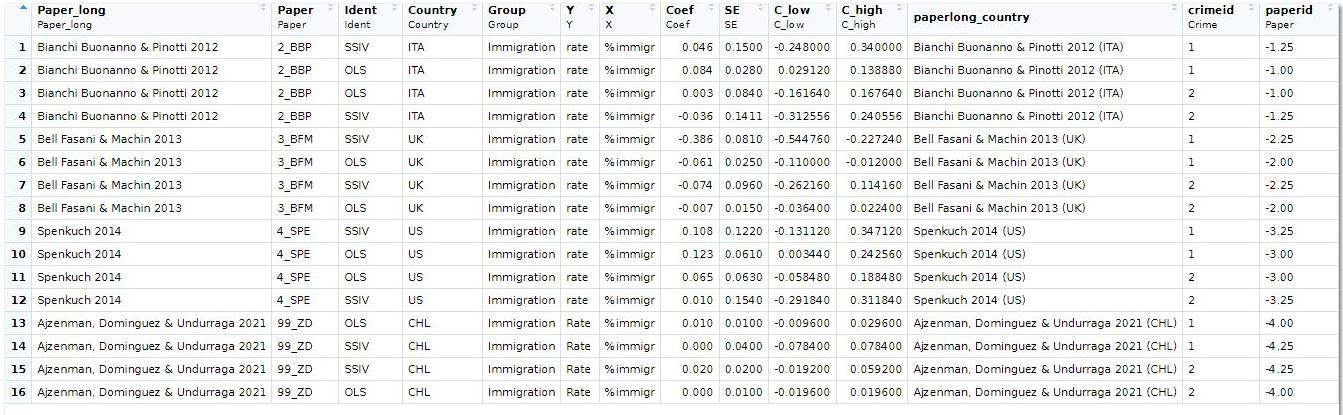
\includegraphics[keepaspectratio]{fig/2.jpeg}}
\end{center}

Image of the Stata File Titled literature.

Once this was done an .xlsx file was created, it was then necessary to
find out which data within the table were used to create the figure. Due
to the data in the .xlsx file not being too large, it was decided to
first look at the data within the spreadsheet to determine whether it
was possible to understand it, or whether it was best to use Quatro to
parse the information as to what may or may not be relevant as compared
to the figure.

Due to this data being pre-analysed by the authors, it was not necessary
to make any changes to it. Due to this just being a confirmation that
the authors correctly converted their data into a figure, it was not
necessary to worry as to whether the data needed any analyses, or just
to look for the same numbers and labels which were shown in the figure
the authors presented in their paper. For the figure it was determined
that the data used were Coef for the estimated value, and C\_low for the
lower boundary and C\_high for the upper boundary. These, including
other necessary values were decided were the only values necessary to be
kept from the table. The information as to how these labels corresponded
to what was shown in the figure was determined bu matching the numbers
seen in the table to the figure. However, C\_low and C\_high are pretty
self-explanatory, but the fact that the authors decided to use the label
Coef for the estimate could have caused confusion if the number didn't
match. This is another example of why replication studies could be
difficult as authors may use their own labels in their replication
packages which could cause difficulties when trying to replicate other
studies results.

To do this, the select function was used. Gemini recommended changing
the name of the data that was selected from the literature file as
``data\_for\_the\_plot'' most likely to avoid any confusion as to which
data is which. While only selected data was successfully taken from the
table, it was not organised in the best way to create the figure.
Therefore, the tribble function was used to reorganise the data. The
tribble function is a part of the tibble package (which it itself is a
part of the tidyverse ecosystem). This meant that installing the
tidyverse package would include them both. The tribble function would
allow the data to be organised in a row-wise figuration instead of
columns. Once this was successfully done, a step by step process using
Gemini was used to recreate the original figure as closely as possible.

Next, the data was organised in such a way that would particularly fit
the structure and design of the forest plot; \# Ensure `Study' is
ordered correctly for plotting
data\_for\_plot\(Study <- factor(data_for_plot\)Study, levels = c(``ADU,
2021nChile'', ``SPE, 2014nUnited States'', ``BFM, 2013nUnited Kingdom'',
``BBP, 2012nItaly'')) There was some difficulty in getting everything to
align the way the figure looked in the paper, so Gemini recommended
dodging the data in such a way that everything aligned well; \# Define a
common dodging position to slightly offset the lines vertically
dodge\_pos \textless- position\_dodge(width = -0.4) \# Negative width to
put OLS above Shift Share.

Finally, with the assistance of Gemini matching the design to the
original figure, the design, colours and set up were created using
ggplot. Some tweaking was needed to be performed before these values
were achieved to get the data points to align correctly; \# Use
facetted\_pos\_scales from ggh4x to set different x-axis scales per
facet facetted\_pos\_scales( x = list( Category == ``Property''
\textasciitilde{} scale\_x\_continuous( limits = c(-0.6, 0.4), breaks =
seq(-0.6, 0.4, by = 0.2), labels = scales::number\_format(accuracy =
0.1) ), Category == ``Violent'' \textasciitilde{} scale\_x\_continuous(
limits = c(-0.4, 0.4), breaks = seq(-0.4, 0.4, by = 0.2), labels =
scales::number\_format(accuracy = 0.1) ) ) ) + A very closely matching
figure was created, which essentially was the same as the authors had
created. It can be said with great confident that the author's figure
matches the data within their replication package.

\begin{verbatim}
Warning: `position_dodge()` requires non-overlapping x intervals.
`position_dodge()` requires non-overlapping x intervals.
`position_dodge()` requires non-overlapping x intervals.
`position_dodge()` requires non-overlapping x intervals.
\end{verbatim}

\pandocbounded{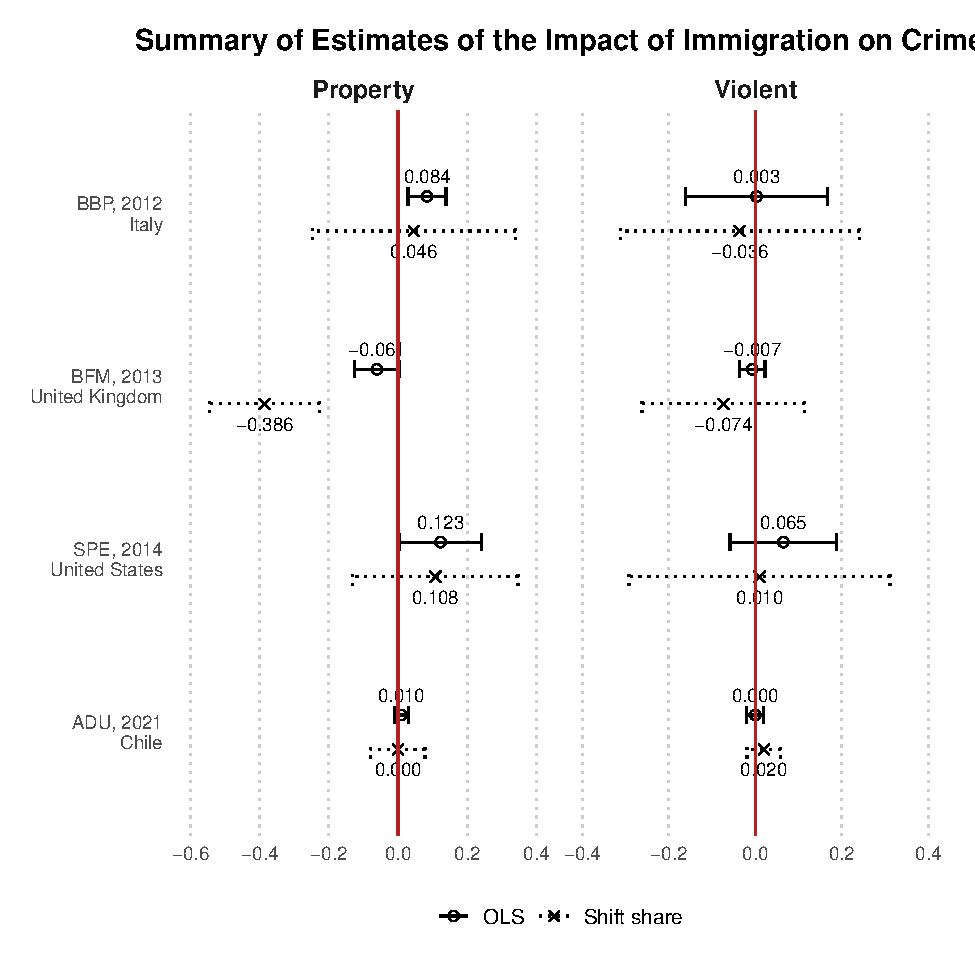
\includegraphics[keepaspectratio]{Replication-Report_files/figure-pdf/unnamed-chunk-13-1.pdf}}

\textbf{Figure~9}\\
\emph{Figure Showing the replicated figure}

\begin{center}
\pandocbounded{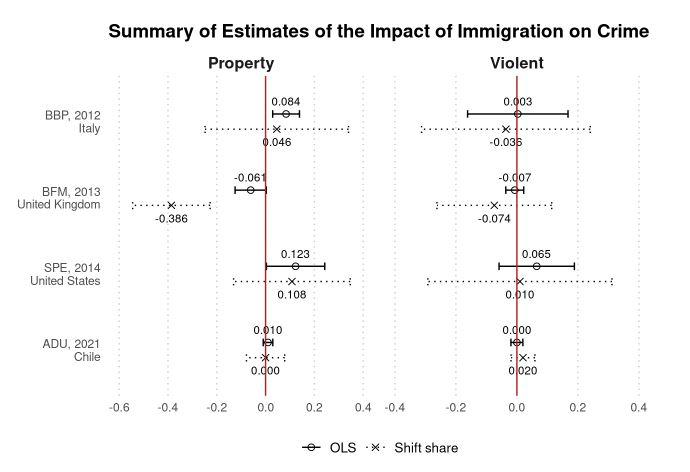
\includegraphics[keepaspectratio]{fig/3.jpeg}}
\end{center}

The next step was to go to the original four papers, retrieve the
original data and then recreate figure 4 again. When choosing the paper
and which figures to replicate, it was confirmed that all the papers
were available with all their data. However, this is where the largest
issue was confronted. Due to each of their papers presenting different
types of data and analysing it in own way, as well as the authors of
this papers using statistical methods which, as well, were only
estimations, this task turned out to be way beyond the scope for this
study. As an example, from the data analysed in the Chile paper
(\citeproc{ref-ajzenman2020}{Ajzenman et al., 2020}) showed the methods
used to analyse their data (Figure 10). The equations they showed are
far beyond the scope that could be reached. Even though it can be seen
in Figure that it is very possible that the data does come from the
paper, such as there being data for robbery, larceny, burglary and
theft, the methods that the Chilean papers used are highly advanced, let
alone the analysis used by the authors of this paper. However, as stated
previously, this is, in its very nature how forest plots operate. They
themselves are used to summarise and meta-analyse more than one study.

\textbf{Figure~10}\\
\emph{Methods and data from} (\citeproc{ref-ajzenman2020}{Ajzenman et
al., 2020})

\begin{center}
\pandocbounded{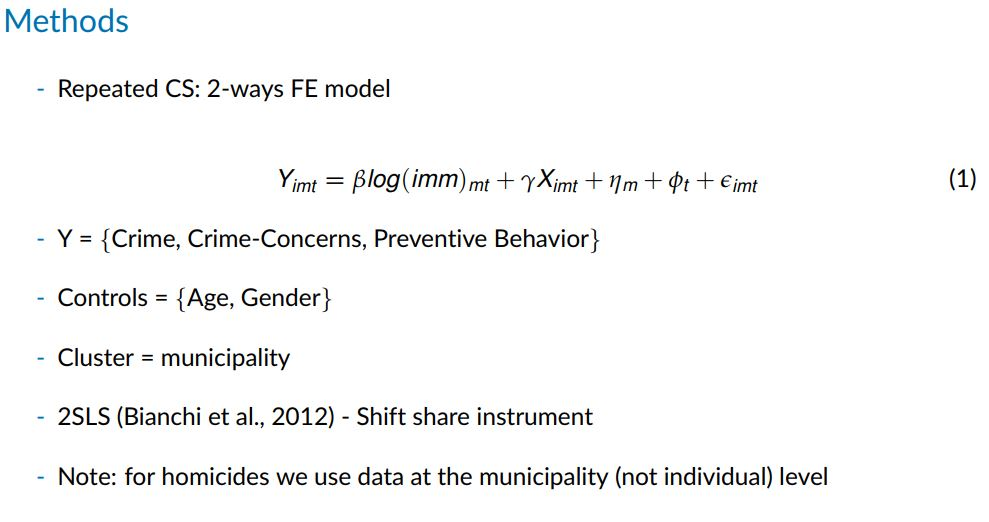
\includegraphics[keepaspectratio]{fig/4.jpeg}}
\end{center}

\begin{center}
\pandocbounded{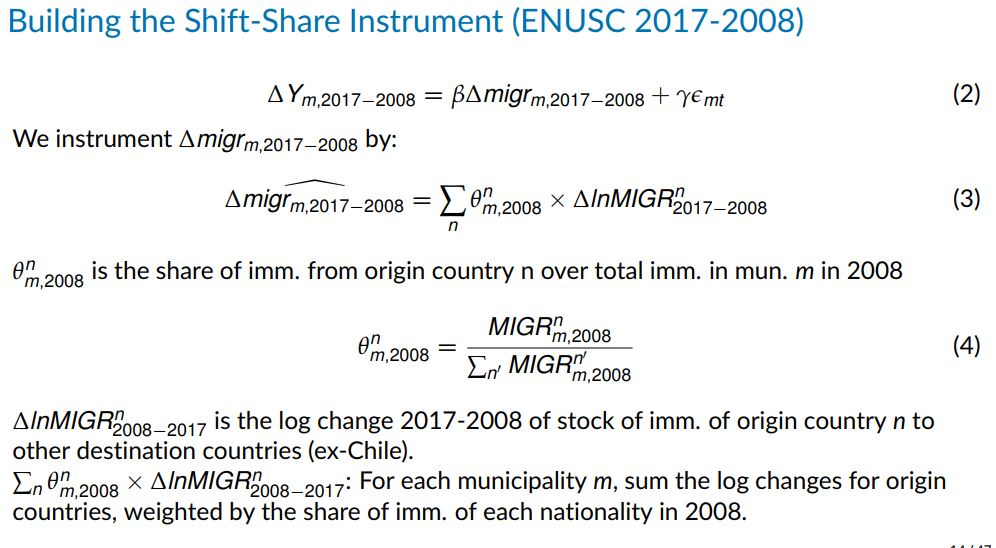
\includegraphics[keepaspectratio]{fig/5.jpeg}}
\end{center}

\begin{center}
\pandocbounded{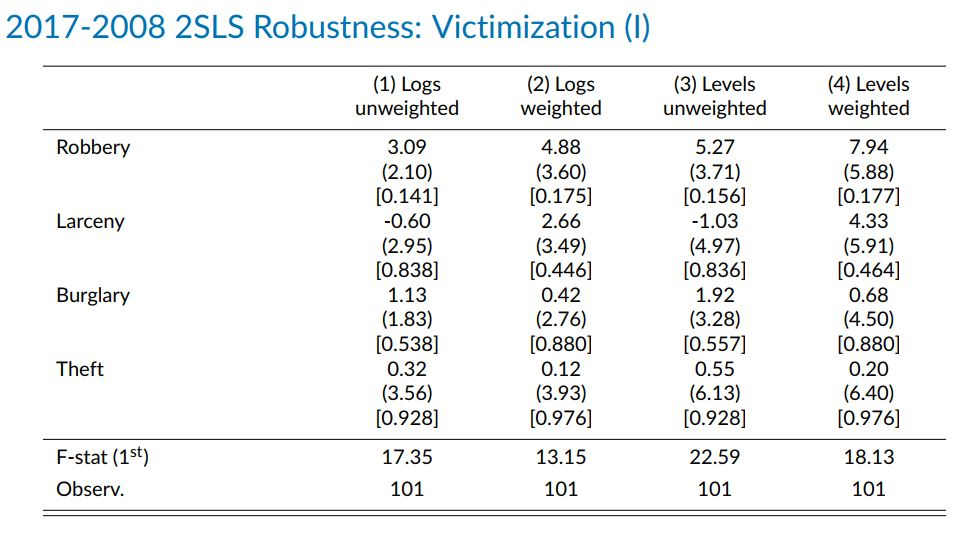
\includegraphics[keepaspectratio]{fig/6.jpeg}}
\end{center}

This should serve as a strong warning that when performing a replication
study, one should be able to perform any analyses or methods that any of
the papers used. While the author's own data here was correctly used in
creating figure 4, the methods they used in creating the shift share
estimates, or even how the primary data was analysed could unfortunately
not be understood. If those performing a replication study are not given
the exact statistical methods used by the authors, it may even be of
importance to contact the original authors to obtain the statistical
methods used in each step, then perform them oneself. However, this is
definitely does not disregard the importance of replication studies in
science. The reproducibility crisis in science is a significant concern,
with many studies facing difficulties in replication
(\citeproc{ref-lobentanzer2020}{Lobentanzer, 2020}).

\subsection{Website Creation}\label{website-creation}

Next was decided to create a website to host the findings and progress
made in creating the reproduction study. Creating a website with the
information obtained from a replication study is a good way to make it
publicly available as to the results of the study.

Initially there was some confusion as how to create a website in RStudio
Cloud, as the initial steps seemed to be quite different as to what was
seen on the Quarto website guide. However, after some Googling, it was
seen that all that needed to be done was to just use R Markdown. It was
decided to just use a simple style in the \_quarto.yml file as shown
below. Then, the figures used in this replication study were separated
to try and make a website that had separated parts. Once the index file
was created, the following website was made.

When following the instructions, and rendering the website in RStudio,
the website appeared to have come out successfully. Therefore, the
information was pushed to GitHub. However, when the website was created
and hosted on the GitHub servers, it appeared to be broken. This was due
to the index.qmd file not being correctly set at the first position.
Instead of -href: index.qmd, it was written as - file: index.qmd. Below
is the correct \_quarto.yml file that was used to create the website.

project:

~ type: website

website:

~ title: ``My Immigration \& Crime: An International Perspective''

~ page-navigation: true

~ sidebar:

~~~ title: Content

~~~ style: `docked'

~~~ contents:

~~~~~ - href: index.qmd

~~~~~~~ text: Home

~~~~~ - href: introduction.qmd

~~~~~~~ text: Introduction

~~~~~ - href: fig2a.qmd

~~~~~~~ text: Figure 2a Data

~~~~~ - href: plot2a.qmd

~~~~~~~ text: Figure 2a

~~~~~ - href: problems2a.qmd

~~~~~~~ text: Problems2a

~~~~~ - href: fig2b.qmd

~~~~~~~ text: Figure 2b Data

~~~~~ - href: plot2b.qmd

~~~~~~~ text: Figure 2b

~~~~~ - href: problems2b.qmd

~~~~~~~ text: Problems2b

~~~~~ - href: fig4.qmd

~~~~~~~ text: Figure 4 Data

~~~~~ - href: plot4.qmd

~~~~~~~ text: Figure 4

~~~~~ - href: problems4.qmd

~~~~~~~ text: Problems4

~~~~~ - href: conclusion.qmd

~~~~~~~ text: Conclusion

format:

~ html:

~~~ theme: cosmo

~~~ css: styles.css

The creation of the \_quarto.yml was assisted with the use of Gemini.
While these AI programs certainly can be a great help, it has to be
strongly noted that they are not perfect programmers, and should
generally be used as assistances as if they introduce an error in your
code, of which you are not familiar with, and may not even be sure how
to ask them the question for them to fix the problem, you may not be
able to resolve it. Having experienced programmers is a better option to
resolve the issue.

When creating the data from R Markdown that will be used to create the
website, it is important all information is organised in the exact
correct order. Because the files used to reproduce the data for the
replication study are in one big file, to make them more presentable on
a website, they must be broken up into the individual pages. Separating
the code does require careful attention to ensure each pages code still
can operate individually. Separating the data (such as text from images
and vice versa), also requires the usage of eval=FALSE (to only keep the
code, but not the data), and echo=FALSE to only keep the figure the data
produces. Performing this allows separate pages allowing for a better
flow. The pages therefore created were as follows;

Home page

Introduction

The data for Figure 2a

Figure 2a

Problems faced in creating Figure 2a

The data for Figure 2b

Problems faced in creating Figure 2b

Figure 2b

Problems faced in creating Figure 2b

The data for Figure 4

Figure 4~~~~~~

Problems faced in creating Figure 4

Conclusion and References.

To publish the website, GitHub pages is used as it freely hosts websites
of a certain size. The following website was then successfully created;

\url{https://tjnh-sci.github.io/tjnh-scigithub.io/}.

This was achieved by first uploading the respective files that will
comprise to a repository. Then going to GitHub Pages and selecting the
location of said files. GitHub Pages has the ability to automatically
recognise the files, and will then publish the website.

\section{Conclusion}\label{conclusion}

Through this replication process and the professor's explanation in
class, I understand the importance of replication for research. It not
only confirms the transparency and credibility of the research, can also
checks whether there are errors or artificial manipulation of data in
the analysis process. The first time I used all the data provided by the
author to make the chart, and only compared the numbers on the website
with the file. The second time I used the data from the World Bank,
although it was under a misunderstanding of the discussion in class,
which resulted in many errors, but on the other hand taught me a lot.

Honestly, after the presentation, I still don't know if it makes sense
for me to use the data from the World Bank, cause I still use the
original calculation of migr\_pop by the author. I asked ChatGPT, and
its answer was: ``If the purpose of your research is just want to see
what happens if you use the WDI population as weight, then it makes
sense to do so: it can answer a new question: If I use the World Bank's
1990 population as weight instead, how will the trend of the global
immigrant share be fine-tuned? This may also be an interesting
robustness check in policy or methodological discussions.'' Seeing the
answer, I was glad that it was not a waste of time. Although using the
World Bank data may not help replicate the graph itself, it's meaningful
to the learning process, and it allowed me to learn how to add the World
Bank data in R and use it correctly.

If I hadn't taken this class, I would have never thought about learning
how to use R or how to write code. I often couldn't understand what the
professor was doing in class, I felt lost in the lecture or I forgott
what to do after Professor finished demonstrating. It started changing
until I had to make this Replication report. At the beginning I did
everything slowly, and when R shows that I had error, I didn't know what
happened. I had to take screenshot and sent it to ChatGPT.Under the
guidance of ChatGPT, I was able to create the graph step by step.
Although I still made a lot of mistakes like the first time I tried to
replicate the graph, I put all the code into the console, and it
worked,the graph showed, but I was not able to keep the code for the
report. When modifying some part of the code, I also made mistakes such
as missing a ) or missing a comma, adding an extra comma, and made an
Incorrect data path etc.Some of the mistakes took me a lot of time to
figure the problems out and fixed them.Lack of familiarity with R often
slows down our progress and was very frustrating.

After I learnt how to create graphs, I even used R to create more graphs
in another group project, which was something I had never expected at
the beginning of the semester, and I am proud of my learning process.

This study study has also shown the importance of taking care in
choosing which studies are chosen and the scope of them. This is not
only important in replication studies, but will be throughout the
thesis.

\phantomsection\label{fig:dhl}
\textbf{Figure~11}\\
\emph{Graph for DHL Project created with R}

\begin{center}
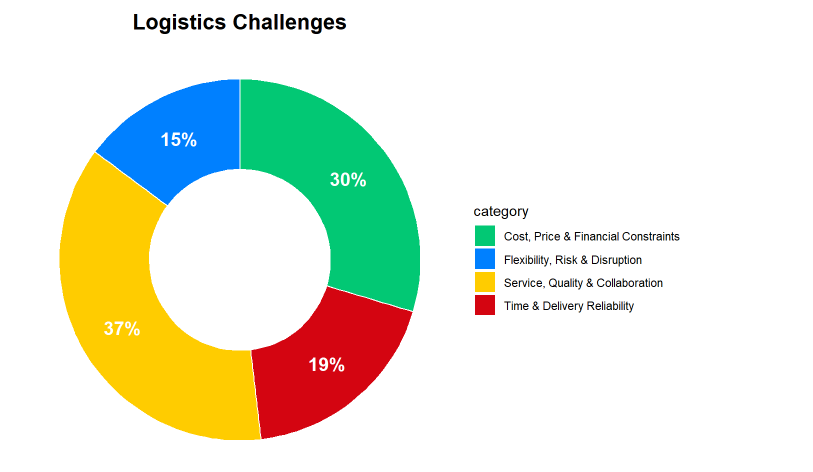
\includegraphics[width=0.8\linewidth,height=\textheight,keepaspectratio]{fig/dhl.png}
\end{center}

\section{Limitations and Future
Directions}\label{limitations-and-future-directions}

The Limitations of this report, we only found data that the author had
cleaned up, which contained the migr\_pop calculated by the authors. We
only compared the total population and murder rate provided by the
authors with the numbers on the websites, and did not download the
original data of these two catagories and recalculate migr\_pop to
verify the numbers provided by the authors.

I think the further direction of this replication study could be to
first use the latest version of immigration data on the UN website for
Figure 2. As I mentioned earlier, the numbers of migration stock are
quite different from the previous version. However, this would involve
recalculating migr\_pop ourselves. second, other violent crimes can also
be included to re-examine the relationship between immigration and crime
rates. Third, use the same analysis method to explore different cities
in a certain country.

\section{The link to presentation}\label{the-link-to-presentation}

\url{https://tjnh-sci.github.io/tjnh-scigithub.io/}

\section{References}\label{references}

\phantomsection\label{refs}
\begin{CSLReferences}{1}{0}
\bibitem[\citeproctext]{ref-ajzenman2020}
Ajzenman, N., Domínguez, P., \& Undurraga, R. (2020). \emph{Immigration,
crime, and crime (mis)perceptions}.
\url{https://doi.org/10.18235/0002714}

\bibitem[\citeproctext]{ref-bell2013}
Bell, B., Fasani, F., \& Machin, S. (2013). Crime and Immigration:
Evidence from Large Immigrant Waves. \emph{The Review of Economics and
Statistics}, \emph{95}(4), 1278--1290.
\url{https://doi.org/10.1162/rest_a_00337}

\bibitem[\citeproctext]{ref-bianchi2012}
Bianchi, M., Buonanno, P., \& Pinotti, P. (2012). Do Immigrants Cause
Crime? \emph{Journal of the European Economic Association},
\emph{10}(6), 1318--1347.
\url{https://doi.org/10.1111/j.1542-4774.2012.01085.x}

\bibitem[\citeproctext]{ref-bouter2021a}
Bouter, L. M., \& Riet, G. ter. (2021). Replication Research
Series-Paper 2 : Empirical research must be replicated before its
findings can be trusted. \emph{Journal of Clinical Epidemiology},
\emph{129}, 188--190.
\url{https://doi.org/10.1016/j.jclinepi.2020.09.032}

\bibitem[\citeproctext]{ref-lobentanzer2020}
Lobentanzer, S. (2020). \emph{Why most pre-published research findings
are false.} \url{http://dx.doi.org/10.31219/osf.io/29jnp}

\bibitem[\citeproctext]{ref-marie2024}
Marie, O., \& Pinotti, P. (2024). Immigration and Crime: An
International Perspective. \emph{Journal of Economic Perspectives},
\emph{38}(1), 181--200. \url{https://doi.org/10.1257/jep.38.1.181}

\bibitem[\citeproctext]{ref-spenkuch2010}
Spenkuch, J. L. (2010). Understanding the Impact of Immigration on
Crime. \emph{SSRN Electronic Journal}.
\url{https://doi.org/10.2139/ssrn.1612849}

\end{CSLReferences}

OpenAI. (2025). ChatGPT {[}Large language model{]}.
https://chat.openai.com/chat

\appendix

\section{}\label{}

\section{}\label{apx-a}

\phantomsection\label{fig:checklist}
\begin{center}
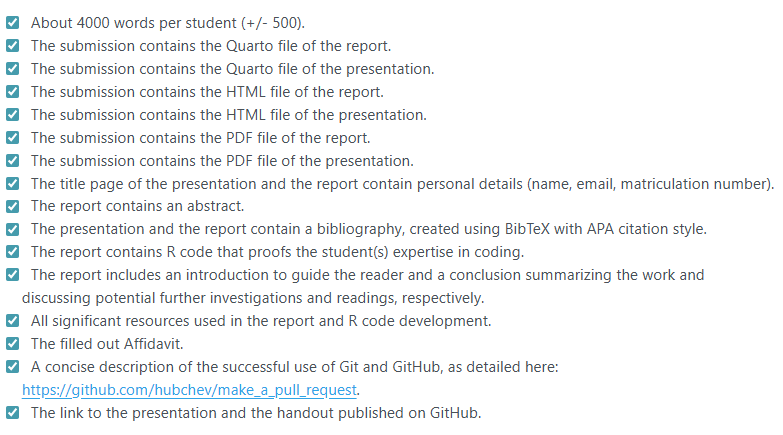
\includegraphics[width=1\linewidth,height=\textheight,keepaspectratio]{fig/checklist.png}
\end{center}

Yu-Chiao Tseng 21. July. 2025 Cologne Tawanda Nhundu 21. July. 2025
Cologne






\end{document}
